\documentclass[12pt]{article}
\usepackage{paper,math}
\usepackage[margin=1in]{geometry}
\addbibresource{references.bib}

\title{Genomorientierte Bioinformatik \\ Report \\ Read Simulator}
\author{Malte Weyrich}
\date{\today}
% Conditionally display thoughts (hide by switching to `\boolfalse`)
% \booltrue{INCLUDECOMMENTS}
\newcommand{\malte}[1]{\coauthorComment[Malte]{#1}}

\begin{document}

% Title Page -------------------------------------------------------------------
\maketitle
\begin{abstract}
	In bioinformatics, \textit{\textbf{Sequencing}} is a term used to describe the process of gathering
	genomic data by reading the nucleotides of a DNA molecule. This is done by a \textit{sequencer}.
	There are different types of sequencing techniques (e.g \textit{Illumina} (next generation sequencing), \textit{Oxford Nanopore},
	\textit{Pacbio} (third generation sequencing), etc.)
	and different variants of \textit{sequencing} (\textit{ATAC-seq}, \textit{scRNA-seq}, \textit{ChIP-seq}, ...).
	In this report, we will focus on a \textit{Read Simulator}, which is a tool used to
	simulate the results of a sequencing experiment (in this case, paired-end \textbf{Sequencing} using \textit{Illumina}).
	The program was executed using \textit{"Homo\_sapiens.GRCh37.75.dna.toplevel.fa"} as \textit{Reference Genome},
	its corresponding \textit{fasta index} and its annotation in form of a \textit{Gene Transfer Format}-File (GTF).
	The \textit{Read Simulator} was written in \textit{Java} and will be benchmarked and analyzed by its complexity and correctness.
	The results of the simulator itself will also be discussed in this report.

\end{abstract}

\newpage


% Paper ------------------------------------------------------------------------

% ------------------------------------------------------------------------------
\section{Introduction}\label{sec:intro}
% ------------------------------------------------------------------------------
The simplified process of \textit{Illumina} sequencing is as follows:
Several DNA target sequences get treated with ultrasound
in order to break them down into smaller fragments of a certain length with a certain margin of error (e.g. 200 bp +/- $x$ bp).
These fragments are labeled, placed onto a flow cell, amplified, and sequenced.
This generates an abundance of short reads, which often overlap with each other and contain mutations.
The reads are then aligned to a \textit{Reference Genome} via a \textit{Mapper} like \textit{STAR} in order to determine the original sequence.
The \textit{Read Simulator} is a tool that simulates this process of generating fragments and reads for given transcript sequences.
In our case, we simulate a paired-end sequencing experiment, where we generate two reads for each fragment, one for each end of the fragment.
With a \textit{Read Simulator}, we are able to validate the results of \textit{Mappers} since we know where our reads originated from.
In other words, if a \textit{Mapper} was to incorrectly map a read (generated by our \textit{Read Simulator}) to the \textit{Reference Genome},
we could detect this faulty behavior and see how far off the \textit{Mapper} was to the actual coordinates.
Like this, we could also detect entire regions inside the \textit{Reference Genome} where the \textit{Mapper} struggles in general (e.g. highly repetitive regions).
A downside of the \textit{Read Simulator} is that it assumes a normal distribution of fragment lengths and
their starting position inside the transcript
and a constant mutation rate across the entire read sequences, which in reality is not the case.
However, it is still a valuable tool for testing the performance of other tools.

The \textit{JAR} was executed using the following configuration:
\begin{verbatim}
java -jar readSimulator.jar 
     -length 75 
     -frlength 200
     -SD 80 
     -mutationrate 1.0 
     -gtf "./inputFiles/Homo_sapiens.GRCh37.75.gtf" 
     -fasta "./inputFiles/Homo_sapiens.GRCh37.75.dna.toplevel.fa" 
     -fidx "./inputFiles/Homo_sapiens.GRCh37.75.dna.toplevel.fa.fai" 
     -readcounts "./inputFiles/readcounts.simulation" 
     -od "output"
    \end{verbatim}

% ------------------------------------------------------------------------------

\section{Java Implementation}
\subsection{Logic}\label{sec:logic}
The logic of the \textit{Read Simulator} is split up into four main steps:
\begin{enumerate}
	\item[\textbf{(A)}] \textbf{Read Gene \& Transcript IDs to Simulate}:\\
		The user specifies a \textit{tsv} file containing the gene and transcript IDs of the sequences and the
		amount of reads to simulate for each transcript. The file is passed to the \textit{ReadSimulator}
		via the \texttt{-readcounts} argument. The entries are stored inside a nested \\
		\textit{HashMap<String, HashMap<String,Integer>\hspace{0.1mm}> readCounts} object where
		the first key corresponds to the gene ID and maps to a second map, which maps the transcript ID to the number of reads to simulate.
		This way, we avoid storing the same gene ID multiple times and can easily access the amount of reads to simulate a given transcript.
	\item[\textbf{(B)}] \textbf{Initialize Genome using a GTF-File}:\\
		The \textit{Genome} class is initialized by passing the path of the \textit{Reference Genome} and the \textit{Fasta Index} file to the constructor.
		The path of the \textit{Reference Genome} is used to create a \textit{RandomAccessFile} object, which is used to
		access the large fasta file in a more efficient way by utilizing the indices stored in the \textit{Fasta Index}.
		This will later be used to extract the sequences of genes containing the transcripts we want to simulate reads for.
		The \textit{GTF} file and \textit{readCounts} object are then passed to the \textit{Genome} object to initialize the gene and transcript coordinates.
		Each line of the \textit{GTF-File} is filtered using \textit{GenomeUtils.filterLine(line, readCounts)}, which
		 checks if the gene ID of the line is present in the \textit{readCounts} object.
		The method works by counting the number of seen \textit{<tabs>} in the current line and then extracting the gene ID,
		which is located in between the 8th and 9th \textit{<tab>} of the line. This way, we don't
		call expensive \textit{split()} operations on each line of the \textit{GTF-File}.
		If a valid line was found, we only need to check if it is a \textit{"gene"}/\textit{"transcript"}/\textit{"exon"} entry
		and either create a new \textit{Gene}/\textit{Transcript}/\textit{Exon} object. A \textit{Gene}
		can have several \textit{Transcript}'s and a \textit{Transcript} can have several \textit{Exon}'s.
		Due to the filtering of \textit{GenomeUtils.filterLine}, our \textit{Genome} object will only contain \textit{Genes} and
		\textit{Transcripts} we want to simulate reads for.
	\item[\textbf{(C)}] \textbf{Initialize Gene Sequences of Interest}:\\
		In order to simulate reads, we first need to extract the exonic sequences of the \textit{Transcripts}.
		This is done by calling \textit{Genome.initTargetSequences(readCounts)}, which iterates over all \textit{Genes} and
		\textit{Transcripts} in the \textit{readCounts} object. For each \textit{Gene}, we extract its sequence using
		the \textit{RandomAccessFile} object and store it in a \textit{String seq} object. This is done by
		utilizing the start/end coordinates of the \textit{Gene} together with the \textit{Fasta Index}
		to can calculate the byte offset of the \textit{Gene} in the \textit{Reference Genome}
		file and read in the sequence.
		The \textit{seq} object can now be used to concatenate the \textit{Transcript} sequences by
		cutting out the exonic sequences of the corresponding \textit{Transcript} based on their
		start and end coordinates.
		This way, we avoid repeatedly accessing the \textit{Reference Genome} file, which
		is time inefficient due to the large size of the file and the vast amount of \textit{Exons} we need to extract.
		If a \textit{Gene} is located on the reverse strand, we go through the \textit{Exons} in reverse order.
	\item[\textbf{(D)}] \textbf{Generate Reads and Write to File}:\\
		For each \textit{Transcript} we want to simulate reads for, we sample a random fragment length and starting position from a normal distribution.
		These two values and the specified \textit{read length} are used to extract two substrings of the \textit{Transcript} sequence:
		\begin{verbatim}
do {
    fragmentLength = (int) Math.round(normalDist.sample());
} while (fragmentLength < length || fragmentLength > transcriptSeq.length());
int maxStartPos = transcriptSeq.length() - fragmentLength;
int randomStartPos = splittableRandom.nextInt(maxStartPos + 1);
String fwSeqRead = transcriptSeq.substring(
                        randomStartPos, 
                        randomStartPos + length
                    );
String rwSeqRead = GenomeUtils.revComplement(
                        transcriptSeq.substring(
                            randomStartPos + fragmentLength - length, 
                            randomStartPos + fragmentLength
                        ));
       \end{verbatim}
		These two \textit{Strings} resemble the unmutated forward (\textit{fw}) and reverse (\textit{rw}) sequence of the \textit{Read}.
		The \textit{start/end} positions inside the \textit{Transcript}, the \textit{Read} sequence, the \textit{Read ID} and a \textit{boolean} indicating if the \textit{Read}
		is the forward or reverse \textit{Read}, are then collected in a \textit{Read} object (\textit{fwRead} or \textit{rwRead}).
		We iterate over each nucleotide of the \textit{Read} and use the \textit{mutationRate} to determine if we should mutate the nucleotide of the
		current position.
		Mutations to the original nucleotide are not considered, so we only mutate to one of the other three nucleotides.
		The next step is to derive the \textit{Genomic Region Vector} of both \textit{Reads}.
		In Figure \ref{fig:mapping}, we can see the mapping of the \textit{Reads} to the \textit{Reference Genome} using the prior knowledge of the \textit{Exon} coordinates.

		\begin{figure}[htpb]
			\centering
			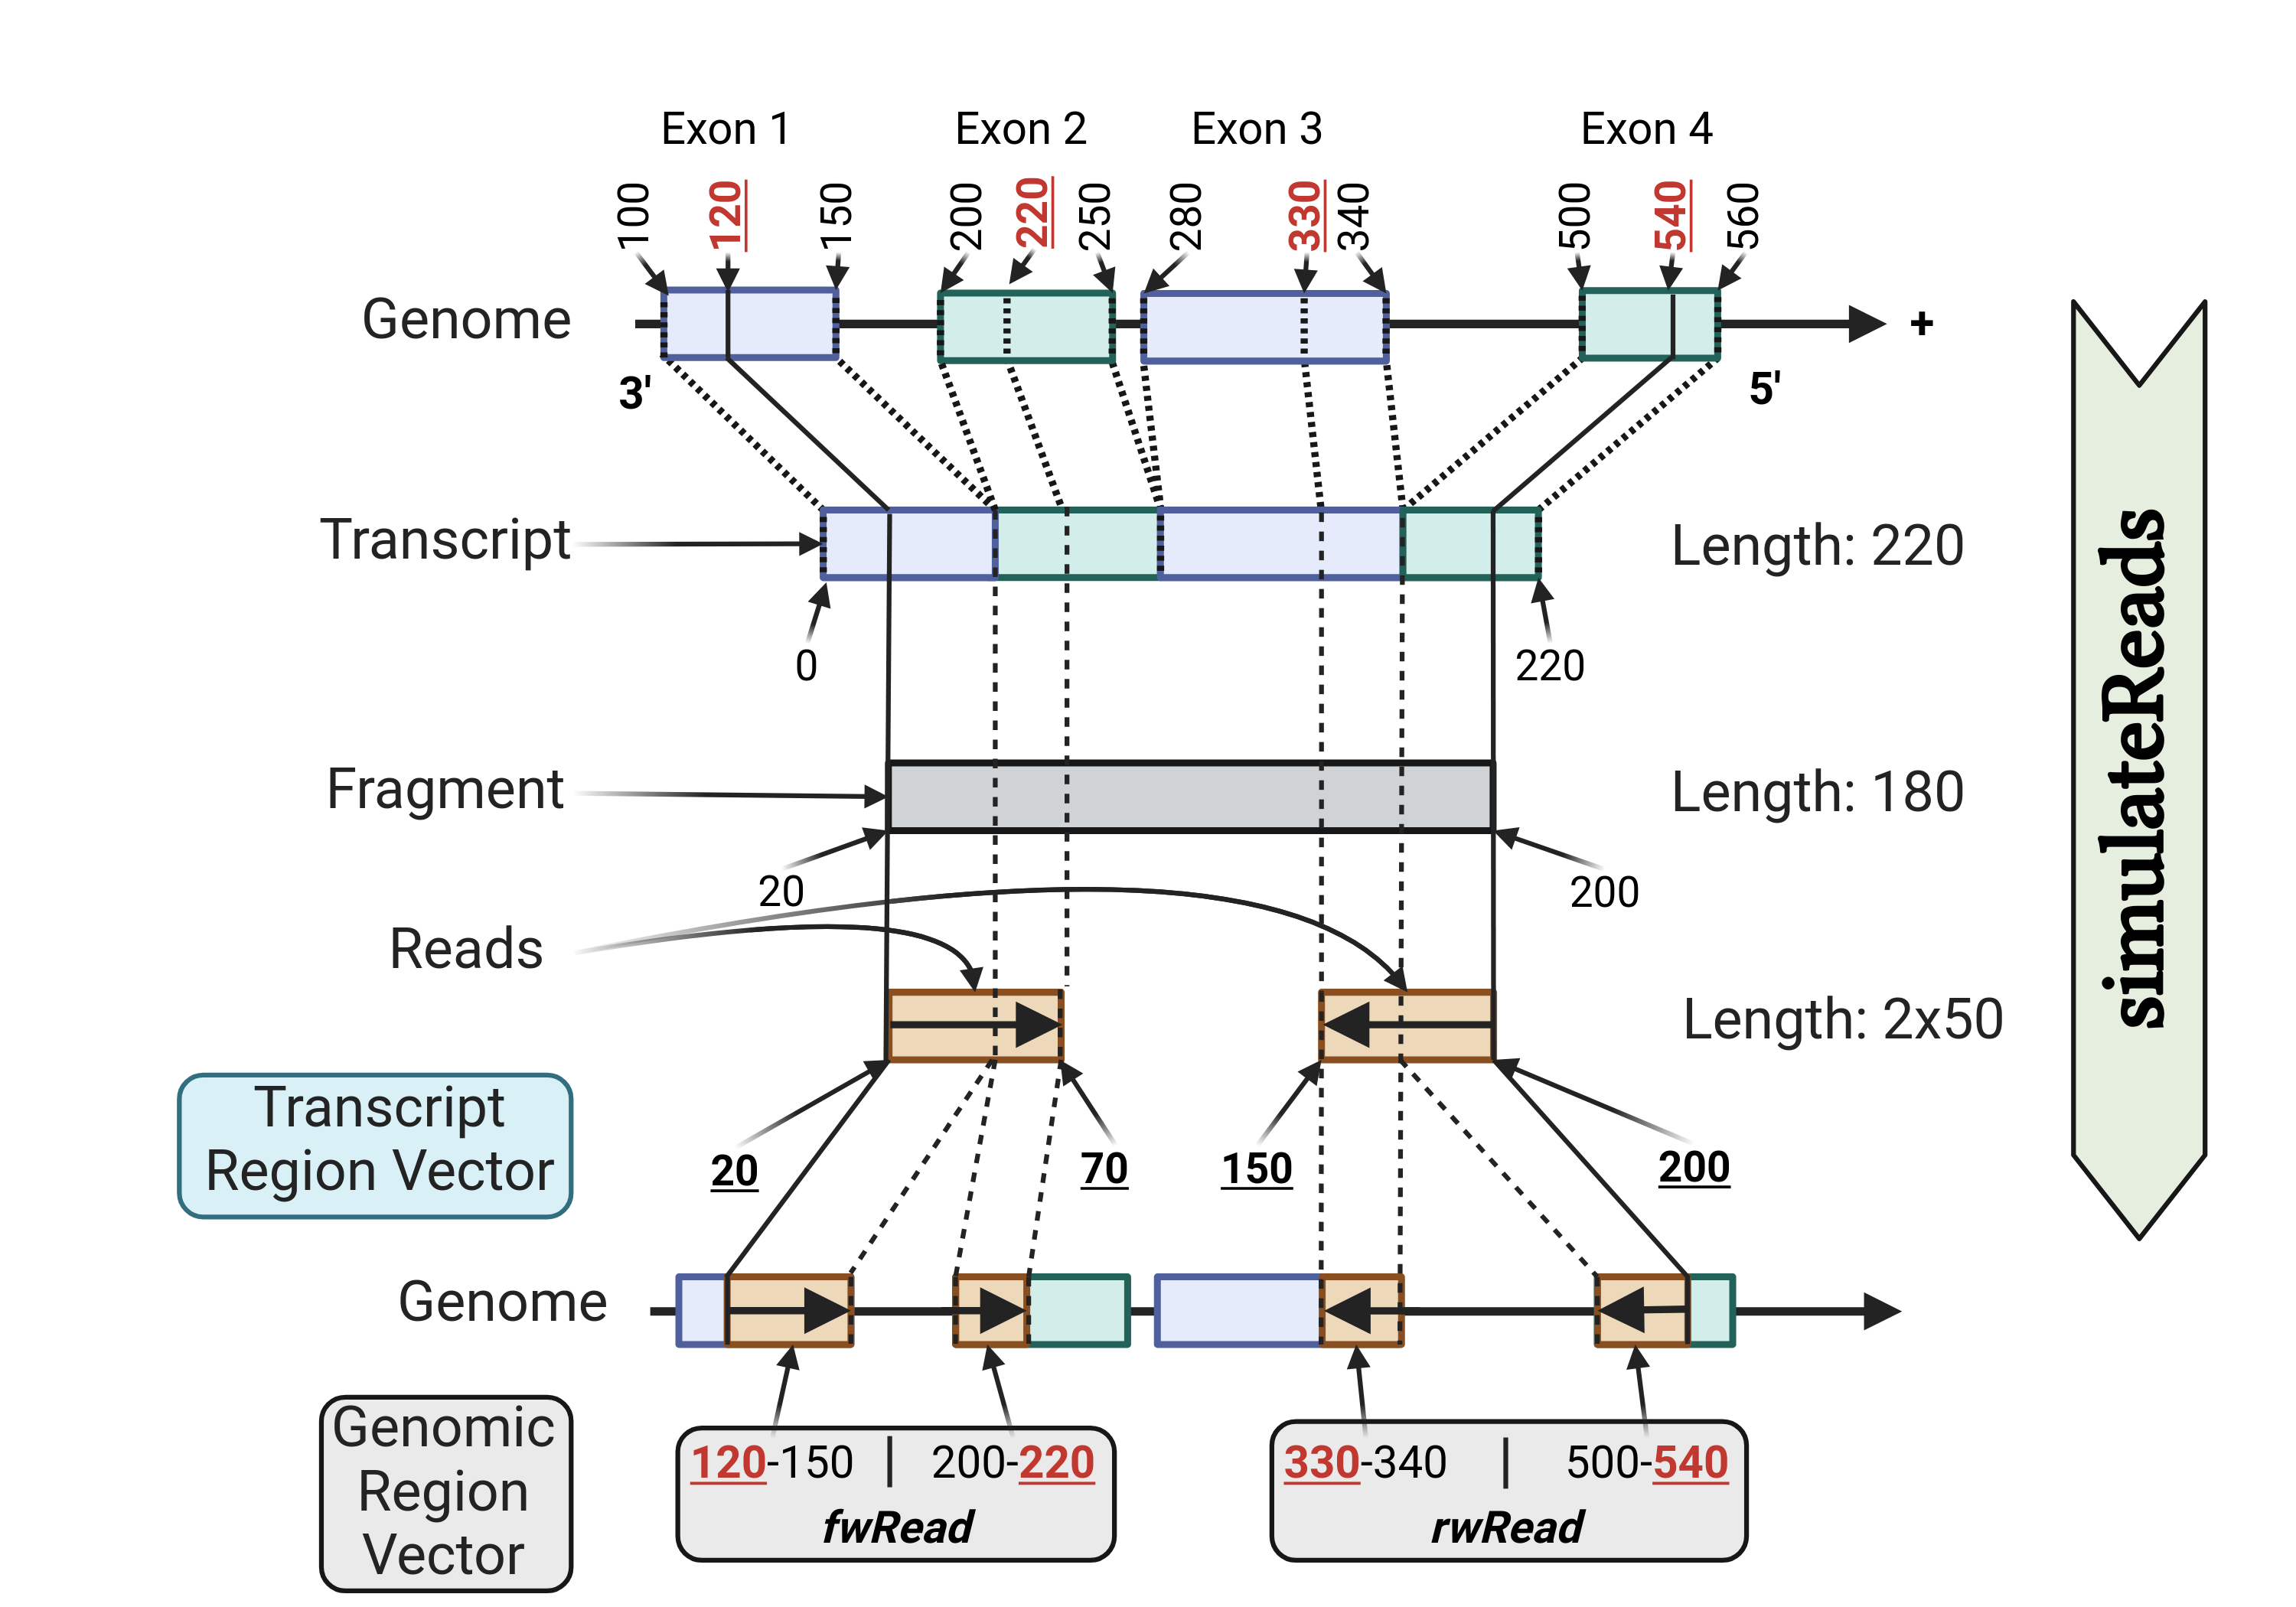
\includegraphics[width=0.95\textwidth]{"./figures/Map.png"}
			\caption{Mapping of Reads (of length 50) to the Reference Genome using prior knowledge. This figure was created using \cite{biorender}.}
			\label{fig:mapping}
		\end{figure}

		The method \textit{getGenomicRegion} is used to annotate the generated \textit{Reads} with the corresponding \textit{Genomic Region Vector}.
		We start by extracting the list of \textit{Exons} from the provided \textit{Transcript} object and getting the
		\textit{Read}’s \textit{start} and \textit{end} positions inside the \textit{Transcript}. For each \textit{Exon}, we calculate its genomic \textit{start}, \textit{end}, and \textit{length}.
		By checking if the \textit{Read} overlaps with the current \textit{Exon} in \textit{Transcript} coordinates, we identify the overlapping region.
		This region is then mapped to genomic coordinates, accounting for the strand direction.
		Finally, the genomic regions are formatted and stored in a list, ensuring proper coordinate ordering for the reverse strand,
		before proceeding to the next \textit{Exon}.

		After both \textit{Reads} have been generated and annotated with their \textit{Genomic Region Vectors}, we write them to two separate \textit{fastq} files
		(\textit{"fw.fastq"} and \textit{"rw.fastq"}) in the following format:
		\begin{verbatim}
@0
CTAAAAGGCGCAAGAGAATGGATGATAGTAGTGTCCTCGAGGCCACACGGGTT...
+0
IIIIIIIIIIIIIIIIIIIIIIIIIIIIIIIIIIIIIIIIIIIIIIIIIIIII...
        \end{verbatim}\label{fastq}
		The \textit{Read ID} is followed by the \textit{Read} sequence and a \textit{+} sign. The quality scores are represented by the \textit{ASCII} characters
		\textit{I} in this case. The quality scores are not considered in the \textit{Read Simulator} and are set to the same value for all \textit{Reads}.
		A summary of the generated \textit{Reads} is also created and written to a \textit{tsv} file (\textit{"read.mappinginfo"}) in the following format (table \ref{tab:summary-format}):


		\setlength{\tabcolsep}{3pt}
		\begin{table}[htpb]
			\centering
			\caption{Format of the Summary File created by the Read Simulator. Each row corresponds to a Read Pair (\textit{fwRead} and \textit{rwRead}).}
			\label{tab:summary-format}
			\small
			\begin{tabular}{|c|c|c|c|c|c|c|c|c|c|}
				\hline
				id    & chr   & gene\_id & transcript\_id & t\_fw\_regvec & t\_rw\_regvec & fw\_regvec & rw\_regvec & fw\_mut & rw\_mut \\ \hline
				\dots & \dots & \dots    & \dots          & \dots         & \dots         & \dots      & \dots      & \dots   & \dots   \\
				\hline
			\end{tabular}
		\end{table}

		The \textit{Read} objects are discarded after writing them to the files in order to save memory.
		Writing is done by three separate \textit{BufferedWriter} objects, one for each file.
		The entries are constructed using three different \textit{StringBuilder} objects, which are then written to the files and reset afterward.

\end{enumerate}
\newpage
\subsection{Complexity}
The complexity of the \textit{Read Simulator} can be broken down into the parts described above:
\begin{enumerate}
	\item[\textbf{(A)}] \textbf{Read Gene \& Transcript IDs to Simulate}:\\
		Section (A) of the \textit{ReadSimulator} scales linearly with the amount of lines ($|L_{sim}|$) in the \textit{tsv} file, since
		we create an entry of each line in the \textit{readCounts} object:
		\[
			\mathcal{O}(|L_{sim}|)
			.\]
	\item[\textbf{(B)}] \textbf{Initialize Genome using a GTF-File}:\\
		Let $L_{gtf}$ be a set of all lines in the provided \textit{GTF-File}.
		Each line $l \in L_{gtf}$ has to be checked by the \textit{filterLine} method $(F)$ of \textit{FileUtils}:
		\[
			\sum_{i=1}^{|L_{gtf}|} F(l_{i})
			.\]
		$F$ iterates over all chars in $l_{i}$ and extracts a substring (\textit{relevantCol}) based on the number
		of observed \textit{<tabs>} and \textit{<spaces>}. All these operations are constant in $\mathcal{O}(1)$.
		Let $\bar{l}$ be the upper limit for the length of a \textit{GTF} entry. In the worst case, all lines
		have the maximum length $\bar{l}$. Then each call of $F$ has less than $\bar{l}$ operations, since we
		stop processing the line $l_{i}$ after constructing the relevant substring. In $\mathcal{O}$-notation,
		$\mathcal{O}(F(l_{i})) \in \mathcal{O}(1)$, since $\bar{l}$ is a constant and $\#$ operations of $F < \bar{l}$.
		For the relevant lines $l_{rel}$ (lines that survived filtering), we perform several
		\textit{split()} operations on the entry, and, based on the entry type, parse the \textit{gene ID}
		or \textit{transcript ID}. Let $P(l_{rel})$ describe the remaining amount of work needed
		for parsing the entry. In the worst case, all lines are relevant and need to be processed with $P$.
		Since all these operations are sequential and tied to the number of lines in the \textit{GTF-File}, the overall complexity of \textbf{(B)} can be
		described with:
		\[
			\sum_{i=1}^{|L_{gtf}|} F(l_{i}) + P(l_{rel}) < \sum_{i=1}^{|L_{gtf}|} F(l_{i}) + P(l_{i}) = \sum_{i=1}^{|L_{gtf}|} c_{1} + c_{2} = |L_{gtf}| \cdot (c_{1} + c_{2}) \in \mathcal{O}(|L_{gtf}|)
			.\]
		\newpage
	\item[\textbf{(C)}] \textbf{Initialize Gene Sequences of Interest}:\label{initTargetSequences}\\
		Let $G$ and $T$ be the set of genes and transcript we want to simulate (stored in \textit{readCounts}) and $E_{max}$ be the largest set of exons of a $t \in T$.
		Let's also assume that each gene has exactly one transcript (worst case, because we need to call \textit{GeneSequenceExtractor.getSequence} for each $t \in T$).

		For each entry $(g, t, counts | g \in G \land t \in T) \in readCounts$, we need to extract the gene sequence of $g$.
		This happens by calculating the \textit{offset} ($\in \mathcal{O}(1)$) and reading in the sequence of length $n$ ($\in \mathcal{O}(n)$).
		Let's define $n_{max}$ as the longest gene sequence.
		After extracting the sequence, the transcript sequence needs to be initialized by iterating over its exons.
		We can use $E_{max}$ as an upper limit for this.
		Using these variables, the complexity can be described with:
		\[
			\sum_{i=1}^{|readConts|} n_{i} + |E|_{i} < \sum_{i=1}^{|readConts|} n_{max} + |E_{max}| \in \mathcal{O}\Big(|readCounts| \cdot (n_{max} + |E_{max}|)\Big)
			.\]
	\item[\textbf{(D)}] \textbf{Generate Reads and Write to File}:\\
		At this stage of the program, all transcript sequences have been initialized, and all that's left is to simulate the reads.
		Let $R$ be the sum of all \textit{count entries} of the \textit{readCounts} object, meaning $R$ is the total number of reads to
		simulate. For each read, we need to:
		\begin{enumerate}
			\item[\textbf{(CUT)}] Cut out a random fragment of the transcript
			\item[\textbf{(GEN)}] Generate two substrings stemming from that fragment (\textit{fwSeqRead, rwSeqRead})
			\item[\textbf{(MUT)}] Mutate these substrings
			\item[\textbf{(WRT)}] Write reads to result files
		\end{enumerate}
		Let $e$ be the summary content per line. We can formulate the above into the following expression:
		\[
			\sum_{i=1}^{R} \mathbf{CUT}(frlength) + 2 \cdot \mathbf{GEN}(length) + 2 \cdot \mathbf{MUT}(length) + 2 \cdot \mathbf{WRT}(length) + \mathbf{WRT}(e)
			.\]
		Creating a substring in \textit{Java} with \textit{String.substring()} has a complexity of the length of the substring.
		This means that
		\[
			\mathbf{CUT}(frlength) \in \mathcal{O}(frlength) \land \mathbf{GEN}(length) \in \mathcal{O}(length)
			.\]
		Mutating the reads is also a linear task since we iterate over $length$, and for each iteration, we perform
		constant operations of $\mathcal{O}(1)$:
		\[
			\mathbf{MUT}(length) \in \mathcal{O}(length)
			.\]
		The two \textit{fastq} files generated both contain four lines per read, which is a total of
		\[
			2 \cdot \big(2 \cdot length + 2 + |id|\big)
		\]
		chars. So
		\[
			\mathbf{WRT}\big(2 \cdot (2 \cdot length + 2 + |id|)\big) \in \mathcal{O}(length)
			.\]
		The summary file generated contains one entry $e$ for each read pair. Let $e_{max}$ be the entire with the most chars: $\forall_{e \in entries}: |e| \le |e_{max}|$.
		This means
		\[
			\mathbf{WRT}(e) \in \mathcal{O}(|e_{max}|)
			.\]

		Since $frlength$ and $length$ are fixed constants provided by the user and because $e_{max}$ is
		also a finite upper bound, the overall runtime complexity is:

		\begin{equation*}
			\sum_{i=1}^{R}   \overbrace{\overbrace{\mathbf{CUT}(frlength)}^{c_{1}}  + 2 \cdot \overbrace{\mathbf{GEN}(length)}^{c_{2}}  + 2 \cdot \overbrace{\mathbf{MUT}(length)}^{c_{3}}  + 2 \cdot \overbrace{\mathbf{WRT}(length)}^{c_{4}}  + \overbrace{\mathbf{WRT}(e_{max})}^{c_{5}}}^{C}\\
		\end{equation*}
		\begin{equation*}
			\iff \sum_{i=1}^{R} C = R \cdot C \implies \mathcal{O}(R \cdot C) \in \mathcal{O}(R)
		\end{equation*}


\end{enumerate}

\subsection{Correctness}
The user can provide two additional flags to the \textit{JAR}:
\begin{enumerate}
	\item[I.] \textit{-debug}\\
		If \textit{-debug} is provided, the \textit{JAR} will try to validate all \textit{GenomicRegionVectors} by comparing the current (non-mutated) read sequence
		to a reference sequence. The reference sequence is created by iterating over all coordinates of the corresponding \textit{GenomicRegionVector}.
		This is done for both the \textit{fwRead} and \textit{rwRead} objects. If a single read sequence does not match the reference sequence,
		the \textit{JAR} throws a \textit{RuntimeException} and provides the user with the relevant debug information.
        Additionally, it will also check if all reads are generated. If not, the \textit{JAR} will throw a \textit{RuntimeException}.

	\item[II.] \textit{-transcriptome <pathToTranscriptome>} (in combination with \textit{-debug})\\
		If the user additionally provides a path to a transcriptome corresponding to the input files (\textit{GTF-File}, \textit{fasta}, \textit{fidx}), the \textit{JAR} will
		test all generated transcript sequences (Step \textbf{(C)}) by comparing them to the correct sequences of the transcriptome. If a mismatch
		occurs, the \textit{JAR} will also throw a \textit{RuntimeException}, otherwise a debug statement will be printed.
        This debug case ensures that our \textit{GenomicSequenceExtractor} is working correctly and that the sequences of the transcripts are extracted correctly.
\end{enumerate}
\hspace{0.1mm} \\
If these two debug tests pass, we ensure that the generated reads and their \textit{GenomicRegionVectors} are correct (based on the provided input files).
Using the plots in Section \ref{sec:results}, we can also see that the fragment length and starting position of the reads are distributed as expected.
Conclusively, we can say that the \textit{Read Simulator} is correct.


\newpage

\subsection{Benchmarking}
Steps \textbf{(B) - (D)} were benchmarked by executing the \textit{readSimulator JAR} 30 times using the parameters defined in Section \ref{sec:intro}.

% 30 times 
% GTF 1651ms
% ITG 174ms
% GR 23906ms

\begin{figure}[htpb]
    \centering
    \includegraphics[width=0.8\textwidth]{"./plots/times.jpg"}
    \caption{Mean \textit{JAR} performance in ms after 30 executions measured on \textit{AMD Ryzen 7 PRO 4750U with Radeon Graphics (16) @ 1.700GHz}.}
    \label{fig:plots-times-jpg}
\end{figure}

Figure \ref{fig:plots-times-jpg} shows us that generating the reads takes significantly longer than the other steps. This was expected since
the \textit{JAR} had to simulate 7,777,500 reads per run. As described in Section \ref{sec:logic}, the \textit{generateReads} \textbf{(D)} method
does several jobs at once (generating reads, mutating them, and writing them). Usually one would prefer to split these tasks into several 
smaller methods, but due to the vast amount of reads generated, it is really memory intensive to do so. Splitting up
\textit{generateReads} would require storing all \textit{Read} objects in a data structure and lead to excessive heap usage.

% generateReads            19.440
% Writer.write             4.739
% mutateRead               3.766
% getGenomicRegion         2.570
% StringBuilder.append()   2.640
% String.join              0.920
% NormalDistributionSample 0.430
% unknown                  4.375 

\begin{figure}[t]
    \centering
    \begin{minipage}[t]{0.45\textwidth} 
        \centering
        \includegraphics[width=\textwidth]{./plots/generateReads_times.jpg} 
        \caption{\textit{generateReads} method\\ analyzed by CPU time using \textit{IntelliJ Profiler}.}
        \label{fig:generateReads-time}
    \end{minipage}
    \hfill
    \begin{minipage}[t]{0.45\textwidth}
        \centering
        \includegraphics[width=\textwidth]{./plots/generateReads_ma.jpg}
        \caption{\textit{generateReads} method\\ analyzed by memory allocations using \textit{IntelliJ Profiler}.}
        \label{fig:generateReads-ma}
    \end{minipage}
\end{figure}
In Figure \ref{fig:generateReads-time} and \ref{fig:generateReads-ma} we can see method \textbf{(D)} split up 
into its components based on \textit{CPU time} and \textit{memory allocations}.
Note that the component \textit{unknown} in Figure \ref{fig:generateReads-time} was the fraction of \textit{generateReads}, which was not 
displayed/identified by the \textit{IntelliJ Profiler}. It is most likely the time needed for garbage collection by \textit{JVM} since each \textit{Read} object
and its \textit{readSeq} object are temporary objects that only exist once per iteration.
The process of writing takes up the second most considerable fraction in this plot, which is due to the 
high amount of information being written (around 3.4GB). Mutating the read sequences is unsurprisingly also 
quite intensive in its time usage. A total of $7,777,500 \cdot 2 \cdot length$ positions need to be mutated ($length ==$ read length), each time 
generating a new random \textit{double} and potentially needing to draw several bases per position (since mutations like 
'A' $\mapsto$ 'A' are not allowed). 
Because each output entry is built via \textit{StringBuilders}, we call \textit{StringBuilder.toString()} three times per read
($3 \cdot 7,777,500$) and each time this happens, new memory is allocated. A total of $4.55 GB$ of allocations can be traced 
back to this cause.
$4.51GB$ is needed to mutate the reads. The method \textit{mutateRead} creates a new \textit{StringBuilder} each time its called and converts said \textit{StringBuilder} to a \textit{String}
at the end of the method. Additionally, \textit{mutateRead} also saves all positions mutated as a \textit{String} inside an \textit{ArrayList<String>} of the 
current \textit{Read} object. Again, since we call this method $2 \cdot 7,777,500$ times and the \textit{StringBuilders} are temporary, 
the memory allocations accumulate significantly, resulting in the observed memory usage of $4.51GB$.

\newpage
\section{Results}\label{sec:results}
Figure \ref{fig:plots-fr_dist-jpg} plots the length of all generated fragments against their total amount. 
Since a fragment can't be shorter than our specified read length, we have a cutoff at a length of $75$. 
As expected, the fragment length follows a normal distribution with the parameters. 
\[
    \mathcal{N}(frlength, \sigma)
.\]
The \textit{standard deviation} $\sigma$ is also provided by the user (see Section \ref{sec:intro}) and in this case,
$\sigma = 80$.

\begin{figure}[htpb]
    \centering
    \includegraphics[width=0.5\textwidth]{./plots/fr_dist.jpg}
    \caption{Fragment length (\textit{frlength}) distribution across all fragments.}
    \label{fig:plots-fr_dist-jpg}
\end{figure}    



\begin{figure}[ht]
    \centering
    \begin{minipage}[t]{0.45\textwidth} 
    \centering
    \includegraphics[width=\textwidth]{./plots/mut_dist.jpg}
    \caption{Distribution of mutation positions inside all reads.}
    \label{fig:plots-mut_dist-jpg}
    \end{minipage}
    \hfill
    \begin{minipage}[t]{0.45\textwidth}
    \centering
    \includegraphics[width=\textwidth]{./plots/mut_amount.jpg}
    \caption{Number of mutated bases inside read sequences.}
    \label{fig:plots-mut_amount-jpg}
    \end{minipage}
\end{figure}

The distribution of mutated positions inside the generated reads seems to be uniformly distributed (Figure \ref{fig:plots-mut_dist-jpg}). 
Each position has the same probability of mutating (in this case: \\ \texttt{-mutationrate 1.0} $ = 1\%$).
Most reads have between zero and three mutated bases (Figure \ref{fig:plots-mut_amount-jpg}); only around 100,000 have more 
than three mutations, with one outlier having nine mutations.

\begin{figure}[htpb]
    \centering
    \includegraphics[width=0.9\textwidth]{./plots/bar.jpg}
    \caption{Breakdown of total reads into split and non-split categories, including subsets with no mismatches or specific thresholds.}
    \label{fig:plots-mut_bar-jpg}
\end{figure}

Figure \ref{fig:plots-mut_bar-jpg} shows additional read feature insights. 
57\% of the generated reads are contained within only one exon (\textit{Non-split Reads}).
Since, in our use case, the \textit{frlength} (200) is relatively short, it is a likely scenario.
Calculating the mean exon length of the \textit{GTF-File} used in this report also validates
this assumption:

\begin{verbatim}
for(Gene g : genome.getGenes().values()) {
    for (Transcript t: g.getTranscriptList()) {
        for (Exon e: t.getExonList()) {
            totalLength += e.getLength();
            totalExons++;
        }
    }
}
System.out.println(totalLength / totalExons);
>>> 256
\end{verbatim}
 
Because there are less \textit{Split Reads} than \textit{Non-split Reads}, the number of observed
\textit{Split (No Mismatches)} is also smaller that \textit{Non-split (No Mismatches)}.

% ------------------------------------------------------------------------------
% \printbibliography
% ------------------------------------------------------------------------------


% ------------------------------------------------------------------------------
% \newpage~\appendix
% ------------------------------------------------------------------------------


\end{document}

